\chapter[\hspace{0pt}模型建立与求解]{{\heiti\zihao{3}\hspace{0pt}模型建立与求解}}\label{chapter4: 模型建立与求解}
\removelofgap
\removelotgap

\section[\hspace{-2pt}问题1:颜色空间转换模型]{{\heiti\zihao{-3} \hspace{-8pt}问题1:颜色空间转换模型}}\label{section3: 问题1:颜色空间转换模型}

\subsection[\hspace{-2pt}模型建立与求解]{{\heiti\zihao{4} \hspace{-8pt}模型建立与求解}}\label{section3: 模型建立与求解}

为求解 BT.2020 空间到显示屏 RGB 空间的最优线性映射矩阵 $M\in \mathbf{R}^{3\times 3}$,我们采样一组代表性 BT.2020 RGB 样本 $\{c_{i}\}_{i=1}^{N}\in [0,1]^{3}$,其色彩向量经过如下映射:
\begin{equation}\label{eq:linear_map}
  c^{'}_{i} = M\,c_{i}
\end{equation}
然后通过预定义的色彩转换矩阵 $M_{BT\rightarrow XYZ}$ 与 $M_{DP\rightarrow XYZ}$ 将源与目标向量映射至 XYZ 空间,并进一步转换至 CIELab 空间,计算感知误差 $\Delta E_{00}$:
\begin{equation}\label{eq:deltaE}
  L(M)=\frac{1}{N}\sum_{i=1}^{N}\Delta E_{00}\bigl(\mathrm{Lab}(M_{BT\rightarrow XYZ}\,c_{i}),\;\mathrm{Lab}(M_{DP\rightarrow XYZ}\,M\,c_{i})\bigr).
\end{equation}

优化目标为:
\begin{equation}\label{eq:opt_obj}
  \underset {M\in \mathbb{R}^{3\times 3}}{\min}\;L(M).
\end{equation}

为求解上述非线性、不可导且可能存在多个局部极小值的优化问题,我们引入差分进化 (Differential Evolution, DE) 算法\cite{price2013differential}。DE 算法以种群为基础,通过变异、交叉和选择操作迭代更新种群,逐步逼近最优解。

\noindent\textbf{(1)参数编码与搜索空间}
将 $M\in \mathbb(R^{3\times 3})$ 展开为9维向量 $\mathbf{x}\in \mathbb{R^{9}}$ ,并定义搜索空间边界为:
\begin{equation}
\begin{aligned}
  &x_{j}\in [-2,2]m\ \ j=1,...,9
\end{aligned}
\end{equation}
\noindent\textbf{(2)初始化种群}
生成 $NP$ 个个体 $\mathbf{x}_{i}^{(0)}\in \mathbb{R^{9}}$:
\begin{equation}
\begin{aligned}
  &x^{(0)}_{i,j}=l_{j}+r_{i,j}\cdot (u_{j}-l_{j}),\ \ r_{i,j}\thicksim \mathcal{U}(0,1)
\end{aligned}
\end{equation}

\noindent\textbf{(3)变异操作}
对第 $i$ 个个体,在不同个体中随机选择 $\mathbf{x}_{r1},\mathbf{x_{r2}},\mathbf{x_{r3}}$ ,构造差分向量:
\begin{equation}
\begin{aligned}
  &\mathbf{v_{i}}=\mathbf{x_{r1}}+F\cdot (\mathbf{x_{r2}}-\mathbf{x_{r3}})
\end{aligned}
\end{equation}
其中 $F\in (0,2)$ 为差分缩放因子。

\noindent\textbf{(4)交叉操作}
构造试验个体 $\mathbf{u_{i}}$:
\begin{equation}
\begin{aligned}
  &u_{i,j}=
  \begin{cases}
    v_{i,j}^{(t)},&\text{if } \mathrm{rand}_j\le CR\text{ or } j=j_{rand},\\
    x_{i,j}^{(t)},&\text{otherwise},
  \end{cases}
\end{aligned}
\end{equation}
其中 $\mathrm{rand}_j\sim\mathcal{U}(0,1)$ 且 $j_{rand}$ 确保至少一维来自 $\mathbf{v}_i^{(t)}$。

\noindent\textbf{(5)选择操作}
通过目标函数比较试验解与当前个体,选择保留更优者:
\begin{equation}
\begin{aligned}
  &\mathbf{x}_{i}^{t+1}=
  \begin{cases}
    \mathbf{u}_i^{(t)},&\text{if } L\bigl(\mathrm{mat}(\mathbf{u}_i^{(t)})\bigr)<L\bigl(\mathrm{mat}(\mathbf{x}_i^{(t)})\bigr),\\
    \mathbf{x}_i^{(t)},&\text{otherwise}.
  \end{cases}
\end{aligned}
\end{equation}

其中,$L(\mathrm{mat}(\mathbf{x}))$ 由式(\ref{eq:deltaE}) 计算。

\noindent\textbf{(6)终止条件}\
满足以下任一条件则终止迭代:
\begin{itemize}
  \item 最大迭代代数 $T_{max}$;
  \item 种群最优个体的目标函数值变化小于阈值 $\epsilon$。
\end{itemize}

最终输出最优映射矩阵 $M^*=\mathrm{mat}(\mathbf{x}_{best})$,其中
\begin{equation}\label{eq:best_solution}
  \mathbf{x}_{best} = \arg\min_{i=1,\dots,NP} L\bigl(\mathrm{mat}(\mathbf{x}_i^{(T)})\bigr).
\end{equation}


综上所述,为优化色彩转换矩阵 $M$,本文选用差分进化算法(DE)。该方法将 $M$ 参数化为9维向量,并在预设的搜索空间边界内进行优化。通过其经典的种群初始化、变异、交叉及选择等核心操作,DE算法能够迭代地搜寻旨在最小化以 $\Delta E_{00}$ 度量的感知色彩差异的解。鉴于目标函数的非线性、不可导以及可能存在多个局部极小值的特性,DE算法的全局优化能力和鲁棒性,使其成为获取高质量色彩映射的有效计算途径。

\subsection[\hspace{-2pt}问题一结果分析]{{\heiti\zihao{4} \hspace{-8pt}问题一结果分析}}\label{section4: 问题一结果分析}

为实现 BT.2020 色域向目标显示屏 RGB 色域的最优映射,本文构建了感知误差最小化的优化模型,目标为在 CIELab 空间中最小化 $\Delta E_{00}$ 感知色差。我们采样了多个 BT.2020 RGB颜色点,并通过线性映射矩阵 $M\in \mathbb{R}^{3\times 3}$ 变换后,转化至目标显示屏空间,再经过标准变换矩阵应设至 XYZ、CIELab 空间,并利用 $\Delta E_{00}$ 公式计算感知误差。

在模型求解过程中,本文采用了差分进化(Differential Evolution, DE)优化方法,对初始映射矩阵进行迭代寻优。为验证我们模型的稳定性,并提供更可靠的性能评价,我们执行了 50 轮随机优化,并统计其性能指标。主要分析结果如下:

\noindent\textbf{(1)感知误差分布分析}

\circled{1} \textbf{$\Delta E_{00}$损失值统计}

图\ref{figure3: 柱状loss}显示了在50次独立优化实验中,各次优化所达成的最终 $\Delta E_{00}$ 损失值分布情况。其中最大值为 1.0183 ,这表明映射结果在感知层面极为接近参考目标。均值为 0.0744 ,标准差为 0.2083 。这表明该基于 $\Delta E_{00}$ 损失函数的差分进化算法在不同采样条件下都能稳定收敛于较小的感知误差区域,并且具有良好的泛化性能以及良好的稳定性和鲁棒性。

\begin{figure}[h]
\centering
\captionsetup{font={small, stretch=1.312}}
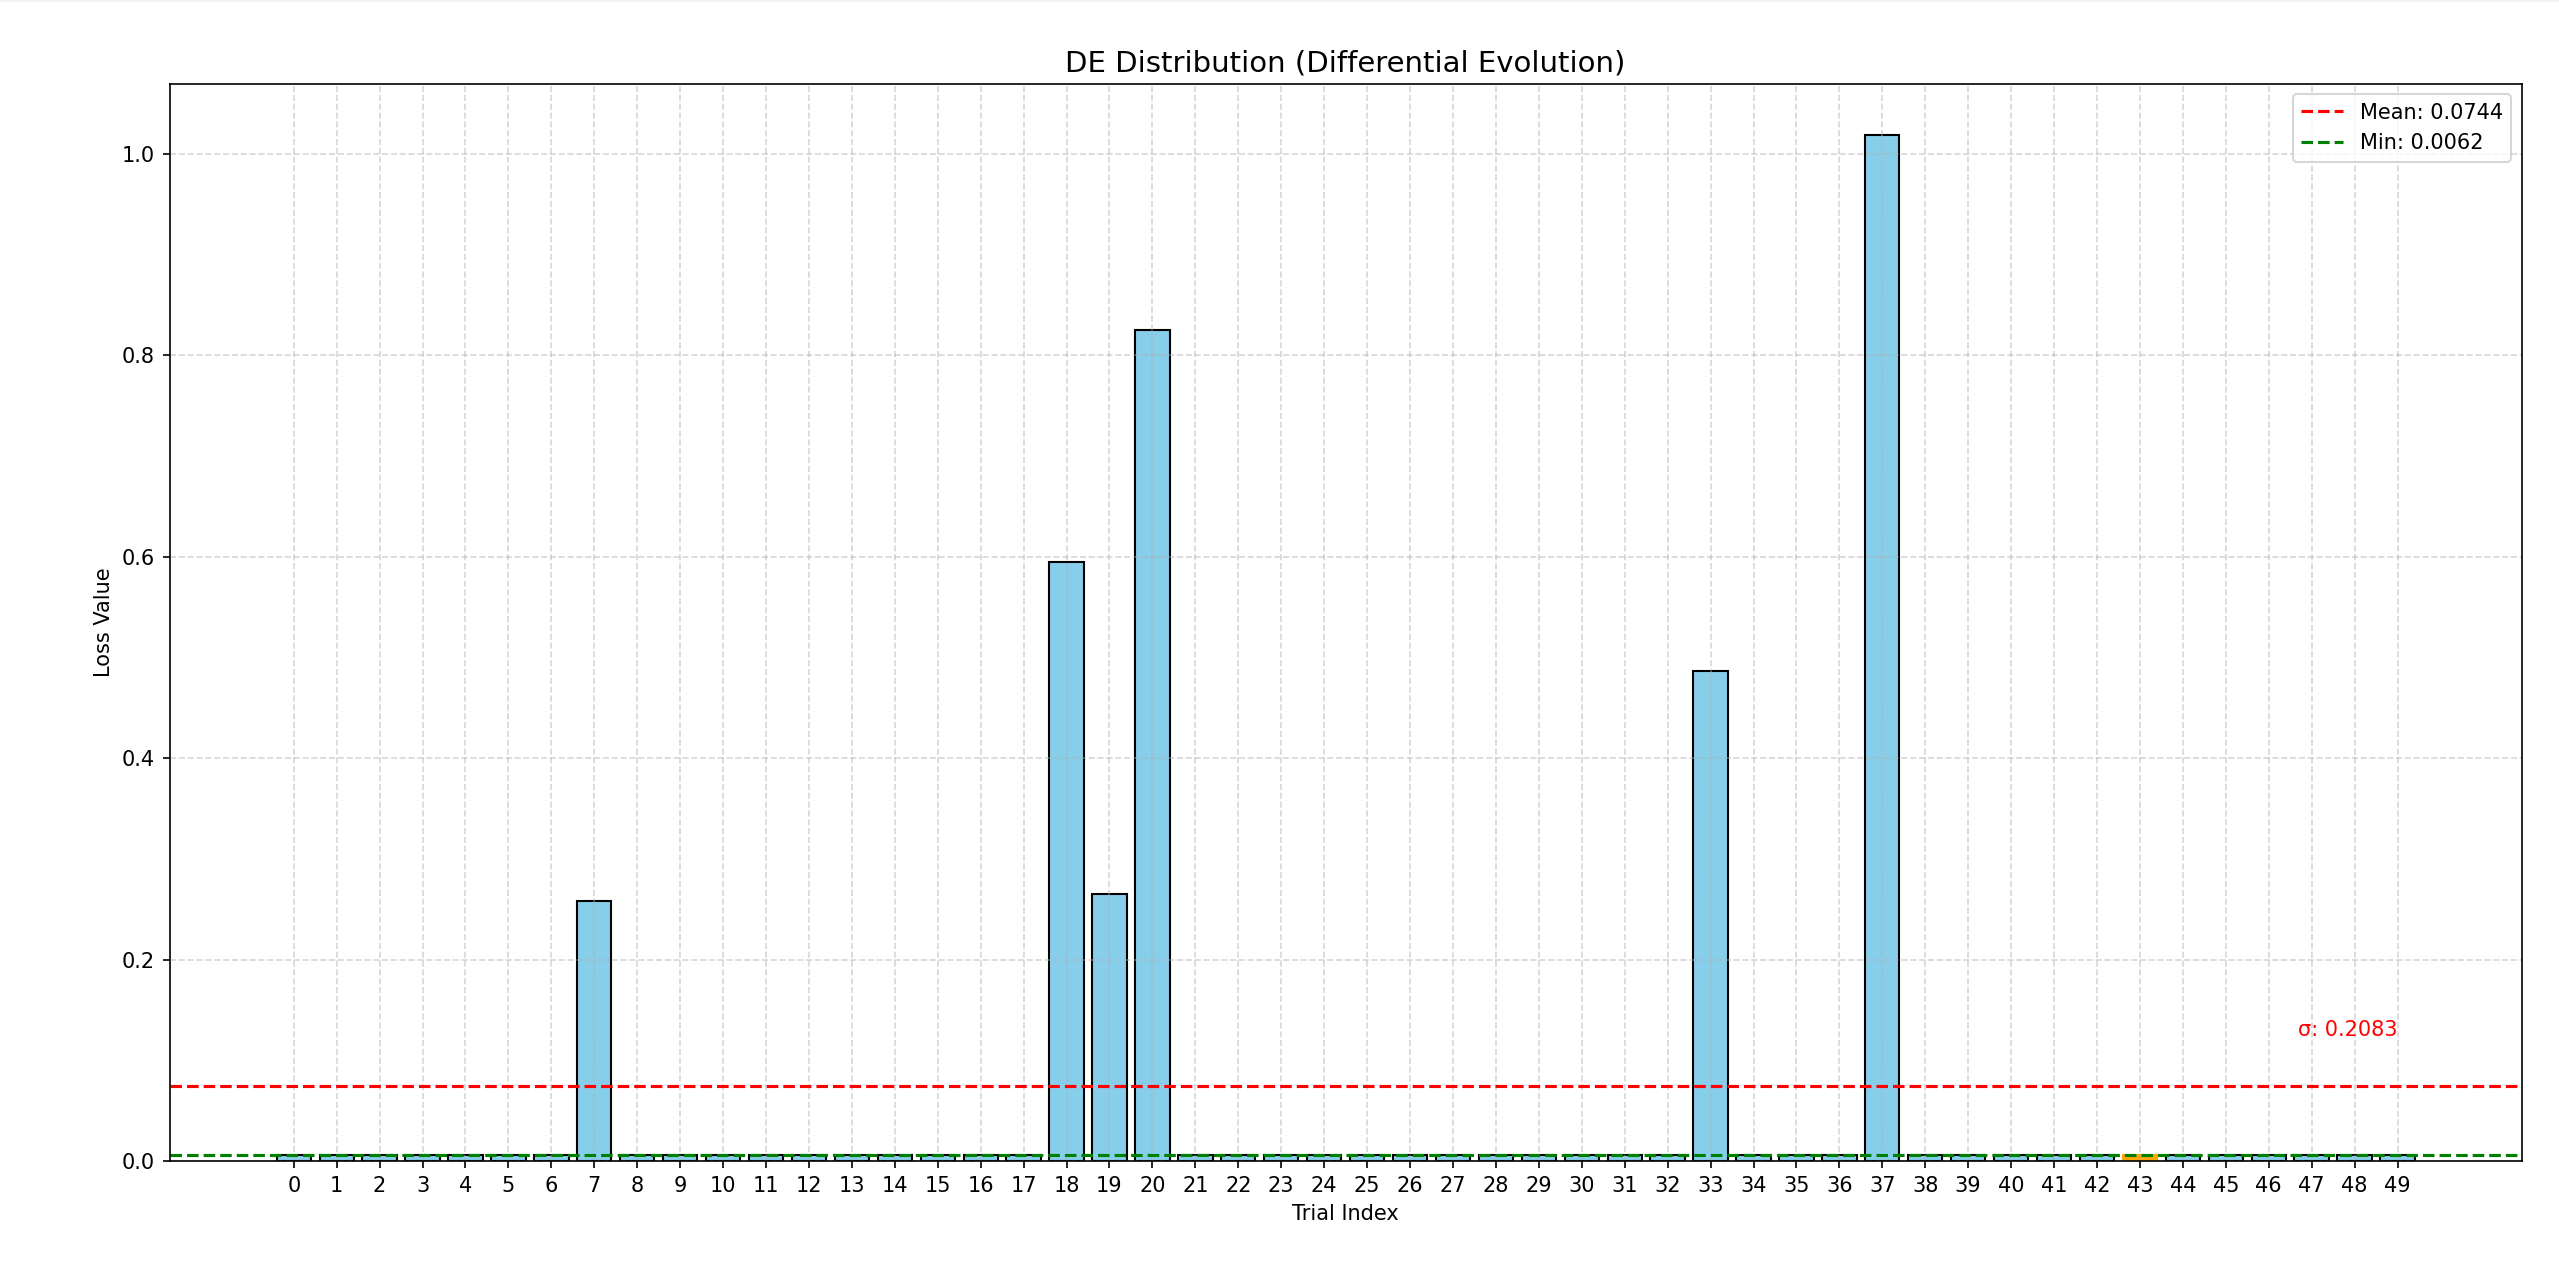
\includegraphics[width=1.0\columnwidth]{figures/DE2000.png}
\bicaption[50次独立优化实验柱状损失图]{50次独立优化实验柱状损失图。}[Histogram of loss values from 50 independent optimization experiments]{Histogram of loss values from 50 independent optimization experiments.}
\label{figure3: 柱状loss}
\end{figure}

\noindent\textbf{(2)色域覆盖度评估}

\circled{1} \textbf{色度空间三角形面积变化}

为评估映射后色域覆盖度变化,我们进一步对比了sRGB 色度三角与模型输出映射后所得的色度三角面积。面积通过三角形在 CIE xy 色度图上的顶点(RGB 基色经映射后的 xy 坐标)计算而得。结果表明,所有 50 次优化中,面积差绝对值均低于 0.001,说明映射后色域几乎无压缩,色彩覆盖极小损失。

\begin{figure}[h]
\centering
\captionsetup{font={small, stretch=1.312}}
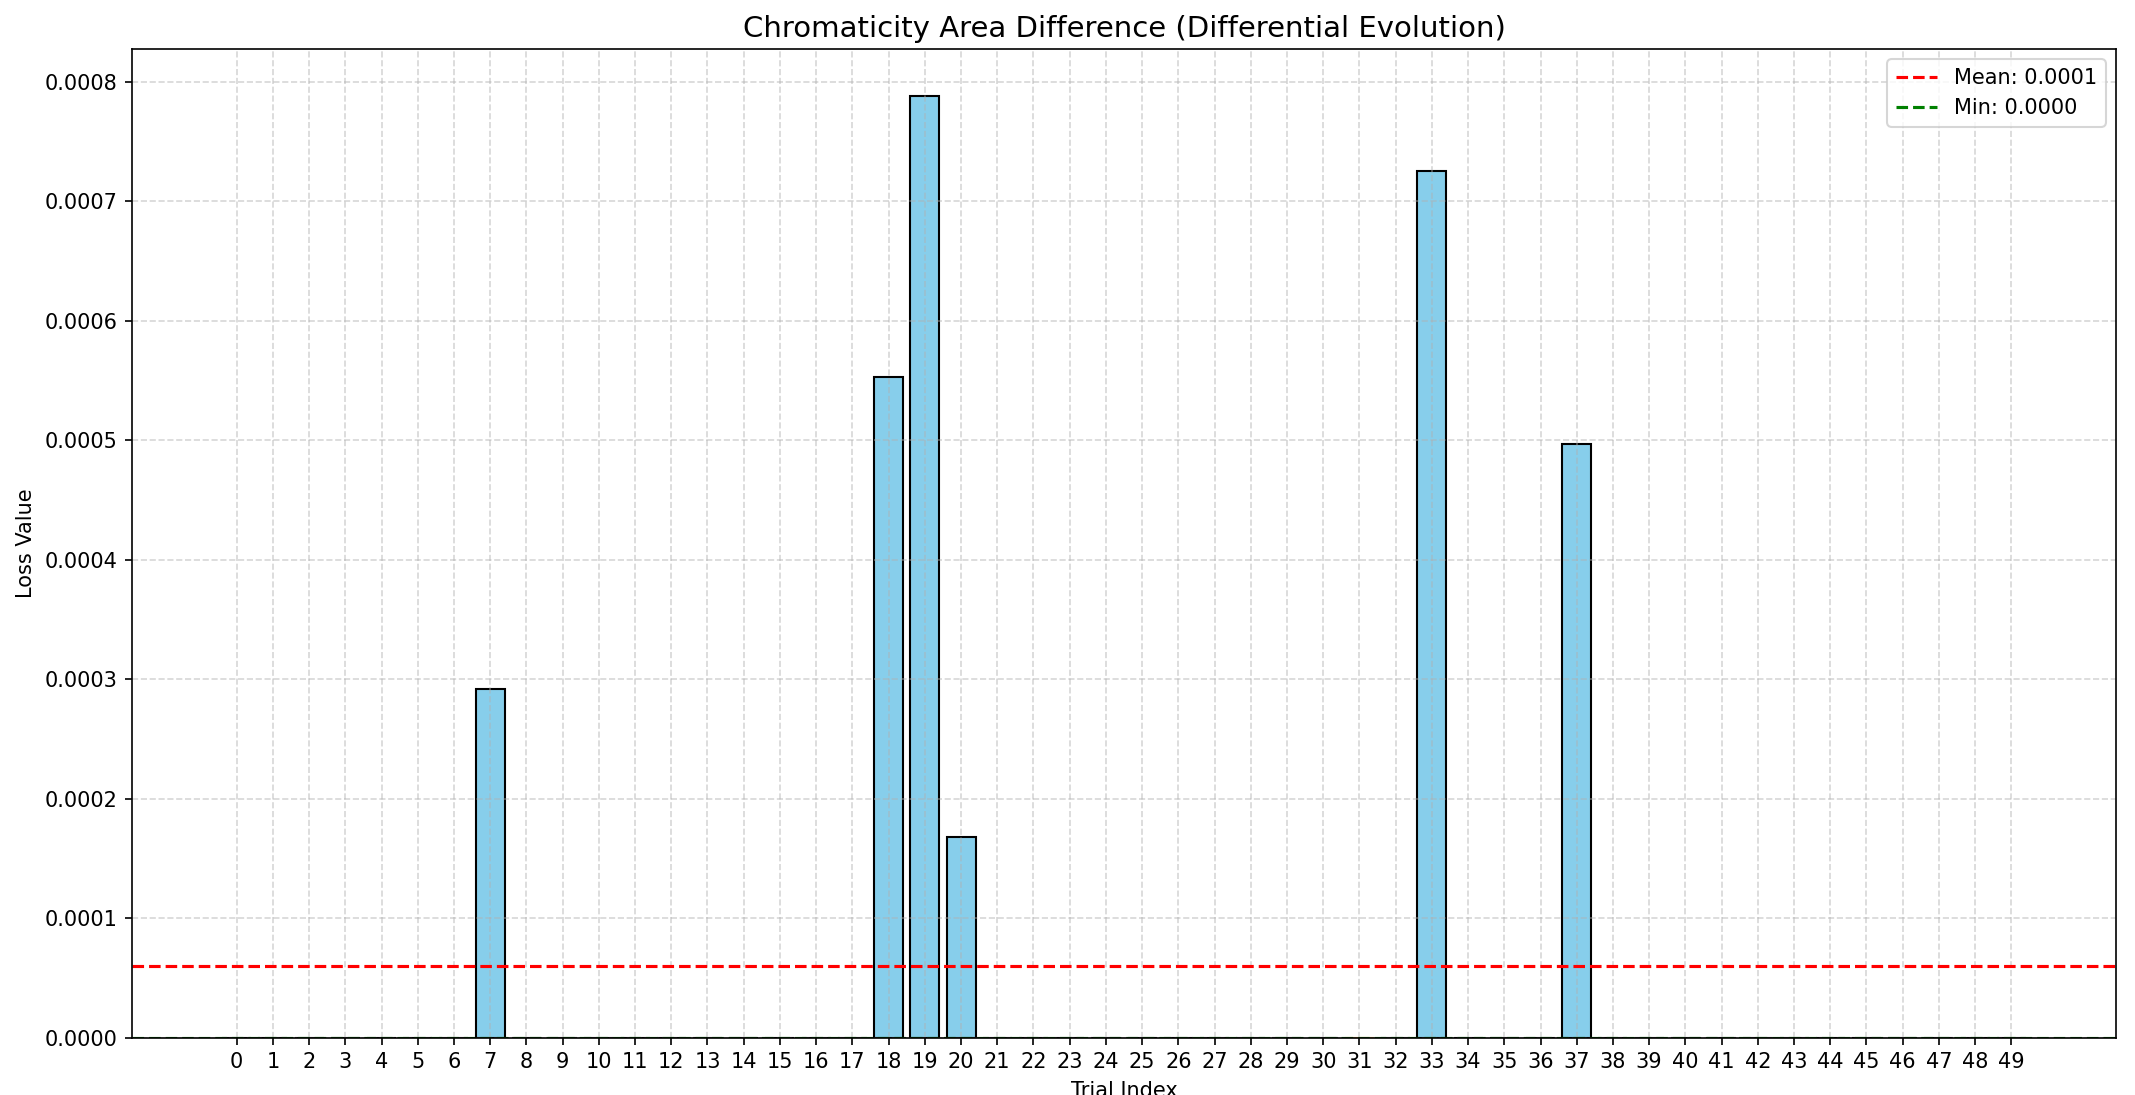
\includegraphics[width=0.8\columnwidth]{figures/面积Loss.png}
\bicaption[50次独立优化实验面积差图]{50次独立优化实验面积差图。}[Area difference plot from 50 independent optimization experiments]{Area difference plot from 50 independent optimization experiments.}
\label{figure3: 面积diff}
\end{figure}

显然我们可以得出,模型在保持色域范围完整性的同时,完成了精准的 RGB 空间映射,并且与 sRGB 的覆盖几乎一致,无明显压缩或扭曲现象。映射后的面积误差控制在 $10^{-3}$ 量级,说明模型不仅保持了色彩准确性,也很好地保留了 BT.2020 色域映射后的覆盖特性。

\circled{2} \textbf{色度图可视化对比}

为直观评估映射效果,我们将 BT.2020、sRGB 以及映射后所得色度三角同时绘制于 CIE 1931 xy 色度图中(见图 3)。可以观察到,模型优化后所得色度三角与标准 sRGB 色域几乎完全重合,进一步验证了在极低感知误差下,实现了对目标色域的高保真拟合。

\begin{figure}[h]
\centering
\captionsetup{font={small, stretch=1.312}}
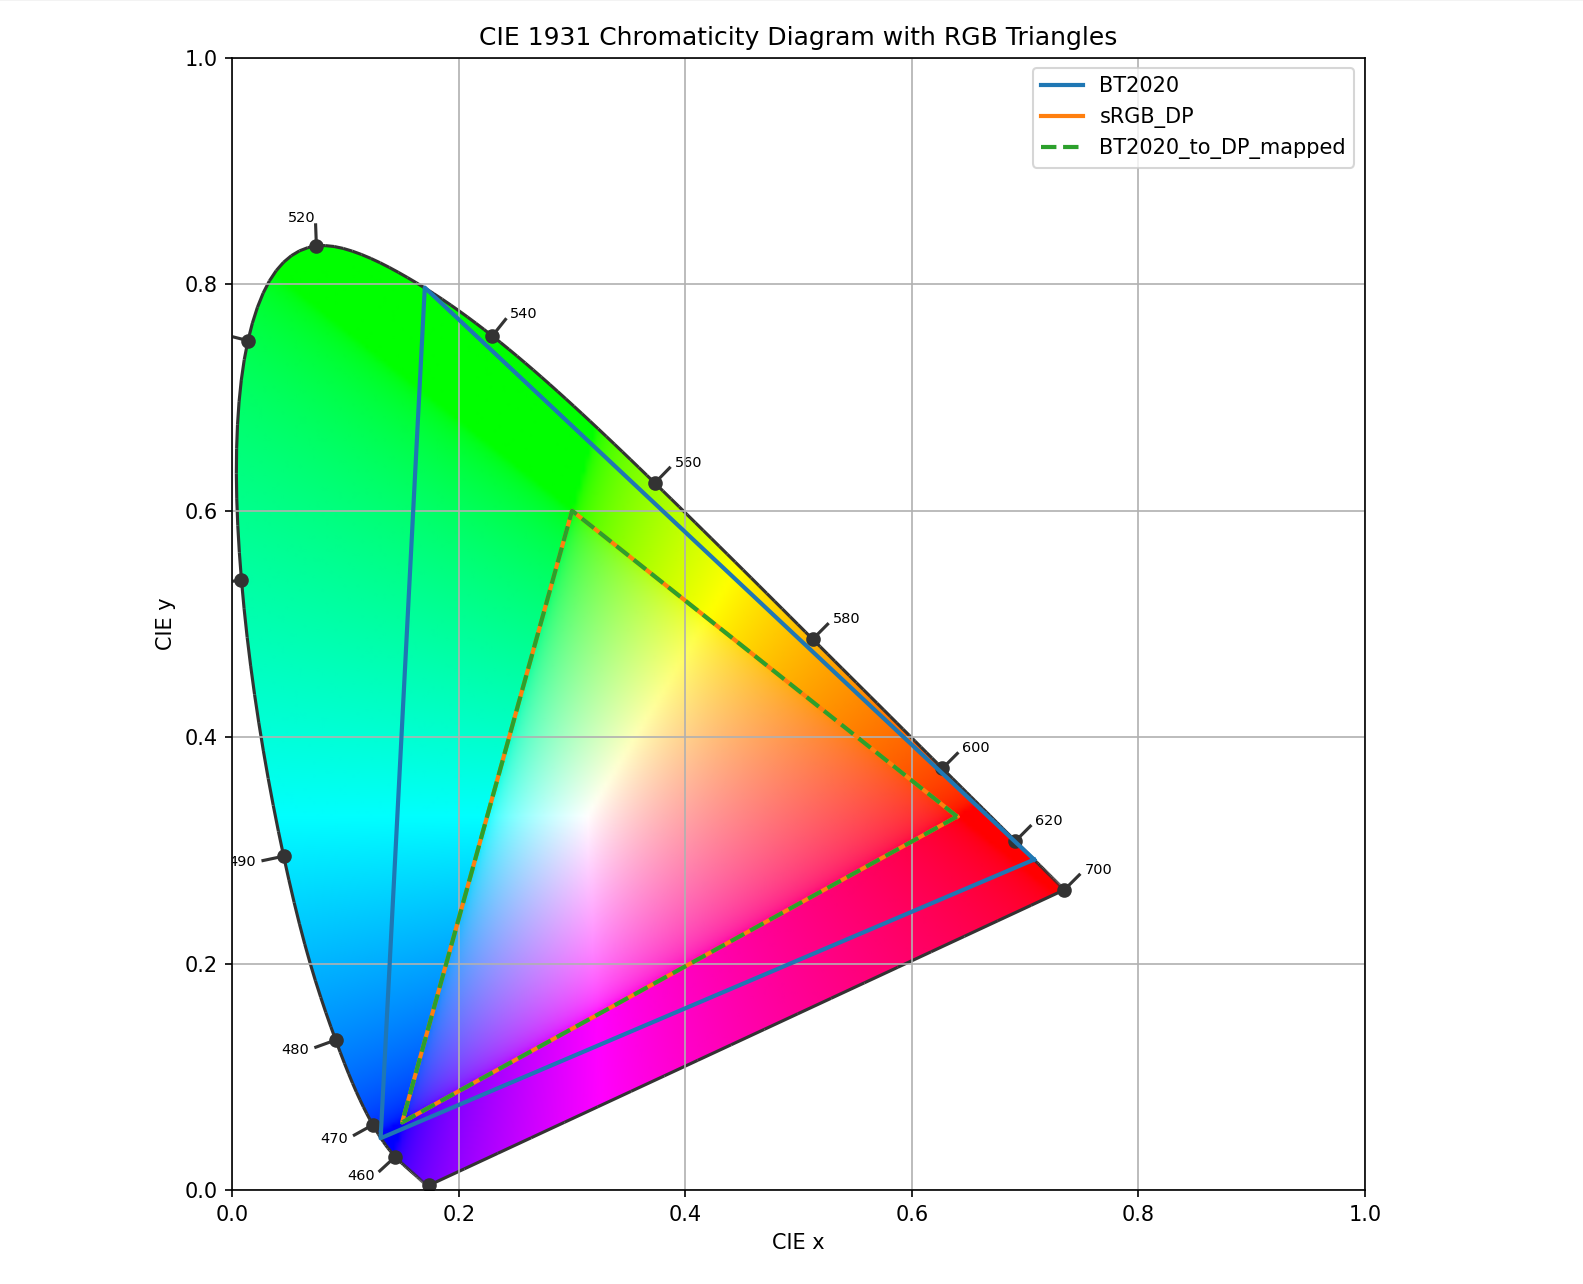
\includegraphics[width=0.8\columnwidth]{figures/色度.png}
\bicaption[色度图]{色度图。}[Chromaticity diagram]{Chromaticity diagram.}
\label{figure3: 色度图}
\end{figure}

\section[\hspace{-2pt}问题2:四通道到五通道颜色转换模型]{{\heiti\zihao{-3} \hspace{-8pt}问题2:四通道到五通道颜色转换模型}}\label{section3: 问题2:四通道到五通道颜色转换模型}

\subsection[\hspace{-2pt}问题分析与建模目标]{{\heiti\zihao{4} \hspace{-8pt}问题分析与建模目标}}\label{section2: 问题分析与建模目标}

本问题旨在解决从 4 通道相机 (RGBV) 到 5 通道 LED 显示屏 (RGBCX) 的颜色空间转换问题。其核心挑战在于:

\noindent\textbf{(1)问题挑战分析}

\circled{1} \textbf{通道数量不匹配}:输入是 4 维,输出是 5 维。这意味着简单的线性变换可能无法有效完成映射,且需要模型能够"创造"出多余的输出通道信息。

\circled{2} \textbf{非线性转换复杂性}:相机捕捉到的 RGBV 信号与显示屏所需的 RGBCX 信号之间通常存在复杂的非线性关系,这可能源于设备响应曲线、环境光照、传感器特性以及显示屏自身的物理特性。

\circled{3} \textbf{感知差异最小化要求}:转换后的颜色应尽可能保留原始颜色的人眼感知,即 $\Delta E_{00}$ 应尽可能小。这是衡量颜色转换质量的关键指标,简单地最小化数值误差可能无法保证视觉效果。

因此,我们的建模目标是建立一个能够将 4 维相机输入(RGBV)映射到 5 维显示输出(RGBCX)的非线性模型,并以最小化颜色感知差异(即 $\Delta E_{00}$)为主要优化目标,同时保证输出值在合理的物理范围内。

\subsection[\hspace{-2pt}神经网络模型设计]{{\heiti\zihao{4} \hspace{-8pt}神经网络模型设计}}\label{section2: 神经网络模型设计}

鉴于颜色空间转换的复杂非线性特性,以及输入输出维度不匹配的问题,我们选择使用前馈神经网络 (Feedforward Neural Network, FNN) 来作为主要的映射模型。

\noindent\textbf{(1)ColorNet架构设计}

我们设计了一个包含多个全连接层的神经网络,其结构如下:

\textbf{输入层}包含4个神经元,每个神经元对应相机捕捉到的一个颜色通道值:红(R)、绿(G)、蓝(B),以及额外的V通道(假设为某种光谱以外的特殊通道或相机特定校准通道)。输入数据直接传入,不进行激活函数处理。

\textbf{隐藏层架构}采用了3个隐藏层,以提供足够的模型容量来学习复杂的非线性映射。第一隐藏层将4维输入映射到64维特征空间,ReLU激活函数$f(x) = \max(0, x)$引入了非线性,使得网络能够学习到非线性特征。第二隐藏层进一步将特征维度提升至128维,增加维度有助于网络发现更丰富的特征组合。第三隐藏层将特征维度降回64维,这种"宽-窄"结构有助于信息在不同抽象层次上的流动和提炼。

\textbf{输出层}包含5个神经元,对应LED显示屏的五个输出通道:红(R)、绿(G)、蓝(B)、青(C),以及额外的X通道(假设为一种补充红色或特定效果通道)。Sigmoid激活函数$f(x) = \frac{1}{1+e^{-x}}$将输出值限制在[0,1]范围内,保证输出的物理合理性。

选择FNN的优势在于其灵活性和通用性。无需对输入输出关系进行复杂的先验假设,FNN可以通过训练自动从数据中学习到最佳的映射方式。多层结构和非线性激活函数使其能够处理高度复杂的颜色转换曲线和相互作用。\cite{1024493909.nh}

\subsection[\hspace{-2pt}损失函数设计]{{\heiti\zihao{4} \hspace{-8pt}损失函数设计}}\label{section2: 损失函数设计}

为了实现模型"最小化感知差异"的核心目标,我们设计了一个混合损失函数 (Combined Loss)。这个损失函数融合了两种不同的误差度量,旨在同时满足数值准确性和视觉准确性。

\noindent\textbf{(1)混合损失函数组成}

我们的混合损失函数由两个主要部分组成:

\textbf{均方误差损失(MSE)}定义为:
\begin{equation}
L_{MSE} = \frac{1}{N} \sum_{i=1}^N \| \text{pred\_rgbcx}_i - \text{target\_rgbcx}_i \|^2
\end{equation}

其中$N$是样本数量,$\text{pred\_rgbcx}_i$和$\text{target\_rgbcx}_i$分别是模型对第$i$个样本的5通道预测输出和真实目标输出。MSE损失确保模型在数值层面接近目标值,有助于网络稳定训练。

\textbf{感知误差损失($\Delta E_{00}$)}定义为:
\begin{equation}
L_{\Delta E_{00}} = \frac{1}{N} \sum_{i=1}^N \Delta E_{00}(\text{pred\_lab}_i, \text{target\_lab}_i)
\end{equation}

其中$\text{pred\_lab}_i$和$\text{target\_lab}_i$分别是模型预测输出和真实目标的RGB部分经sRGB→XYZ→Lab转换后的结果(转换过程详见第\ref{subsection2: CIE1931标准色度观察者与XYZ颜色空间}节和第\ref{subsection2: CIELab颜色空间}节)。$\Delta E_{00}$色差计算采用第\ref{subsection2: CIEDE2000色差公式}节中的标准公式。

$L_{\Delta E_{00}}$是本模型的核心创新点,因为它直接优化了人眼感知的颜色差异。相比于MSE仅关注数值上的匹配,$\Delta E_{00}$损失能够引导模型生成在视觉上更接近目标颜色的输出。

\noindent\textbf{(2)损失函数权重平衡}

总损失函数定义为$ L_{total} = \alpha \cdot L_{MSE} + \beta \cdot L_{\Delta E_{00}} $。在代码中,我们设置了$\alpha=0.1$和$\beta=1.0$。更高的$\beta$值(1.0)表明我们赋予$\Delta E_{00}$损失更高的权重,明确指出我们优先考虑颜色转换的感知准确性。较低的$\alpha$值(0.1)虽然$\Delta E_{00}$是主要目标,但保留一定比例的MSE损失仍然有益,可以提供一个更平滑的优化曲面。通过调整$\alpha$和$\beta$,可以在数值精确度和感知准确度之间找到最佳平衡点,这个平衡点通常需要根据具体的应用场景和视觉要求进行实验和调整。

\subsection[\hspace{-2pt}数据生成与训练策略]{{\heiti\zihao{4} \hspace{-8pt}数据生成与训练策略}}\label{section2: 数据生成与训练策略}

由于实际的 4 通道相机和 5 通道显示屏数据通常难以获取,我们采用了模拟数据生成的方法。

\noindent\textbf{(1)训练数据生成策略}

\circled{1} \textbf{输入数据生成}
\begin{itemize}
    \item 随机生成 $n_samples$ (例如 4000) 个样本,每个样本包含 4 个通道的值
    \item 每个通道的值都在 [0, 1] 范围内均匀随机分布
    \item 这模拟了相机在各种亮度(R, G, B)和特殊通道 (V) 下可能捕捉到的信号
\end{itemize}

\circled{2} \textbf{目标数据生成}
\begin{itemize}
    \item 目标数据的生成旨在模拟一个相对复杂但可控的真实世界颜色转换
    \item 首先,通过一个预设的线性变换矩阵 $W$ 对输入 $X$ 进行加权乘法,得到线性输出 $Y_{linear}$
    \item 接着,在 $Y_{linear}$ 的基础上添加一个非线性扰动,这个扰动项是基于输入 R 通道的一个正弦函数
    \item 最后,将所有输出值裁剪到 [0, 1] 范围,确保颜色通道值保持在物理上合理的范围内
\end{itemize}

\noindent\textbf{(2)模型训练策略}

我们采用了系统化的训练策略来确保模型的有效学习。在优化器选择方面,我们选用AdamW优化器,它是Adam优化器的一种改进版本,在权重衰减(L2正则化)的处理上更为有效,有助于防止过拟合。学习率设置为$5 \times 10^{-4}$,这个学习率是一个常用的起始值,它足够小以避免训练发散,又足够大以保证合理的收敛速度。

在数据处理方面,我们将生成的总数据集按80\%训练集和20\%验证集进行划分,训练集用于模型的参数更新,验证集用于在训练过程中评估模型的泛化能力。训练过程采用小批量(batch size=32)的方式进行,训练数据在每个epoch开始前会进行随机打乱,批次训练有助于提高训练效率、平滑梯度、防止过拟合。

在计算资源和监控方面,模型训练会优先使用GPU(“cuda”)如果可用,否则退回到CPU(“cpu”)。在训练过程中,每隔一定epoch会打印当前的训练损失和验证损失,以便实时监控模型的学习进度和性能。

通过上述详细的模型建立和解析,我们不仅明确了模型的基本架构和关键组成部分,更深入地探讨了其设计哲学和每个组件在解决颜色空间转换问题中的作用,尤其是混合损失函数在平衡数值和感知准确性方面的核心价值。

\subsection[\hspace{-2pt}模型求解和结果分析]{{\heiti\zihao{4} \hspace{-8pt}模型求解和结果分析}}\label{section2: 模型求解和结果分析}

\noindent\textbf{(1)训练过程分析}

\circled{1} \textbf{损失曲线分析}

通过运行训练完成神经网络模型,我们训练了 ColorNet 模型。训练损失曲线展示了模型在训练集和验证集上的收敛情况。

\begin{figure}[H]
\centering
\captionsetup{font={small, stretch=1.312}}
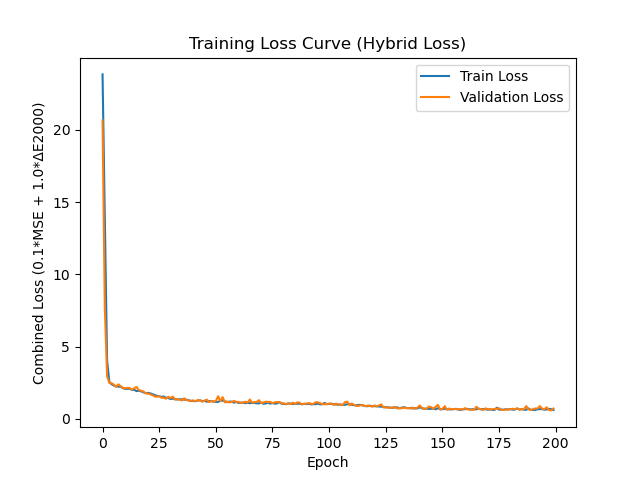
\includegraphics[width=0.8\columnwidth]{figures/Training_Loss_Curve.png}
\bicaption[训练损失曲线(混合损失)]{训练损失曲线(混合损失)。}[Training Loss Curve (Hybrid Loss)]{Training Loss Curve (Hybrid Loss).}
\label{figure2: loss_curve}
\end{figure}

从损失曲线可以看出,随着训练 epoch 的增加,训练损失和验证损失均呈现下降趋势,并最终趋于稳定。为了验证模型的可靠性,我们采用随机生成的数据。模型最终损失值在0.4-0.7之间波动。这表明模型成功地从模拟数据中学习到了 RGBV 到 RGBCX 的映射关系,且没有出现明显的过拟合现象。

\noindent\textbf{(2)感知性能评估}

为了更直观地评估模型的感知性能,我们计算了验证集上预测颜色与目标颜色之间的$\Delta E_{00}$误差,并绘制了直方图和累积分布函数(CDF)。

\begin{figure}[H]
\centering
\captionsetup{font={small, stretch=1.312}}
\includegraphics[width=0.8\columnwidth]{figures/ΔE2000_Error_Histogram.png}
\bicaption[ΔE2000误差直方图(混合损失训练)]{ΔE2000误差直方图(混合损失训练)。}[ΔE2000 Error Histogram (Trained with Hybrid Loss)]{ΔE2000 Error Histogram (Trained with Hybrid Loss).}
\label{figure2: delta_e_histogram}
\end{figure}

\begin{figure}[H]
\centering
\captionsetup{font={small, stretch=1.312}}
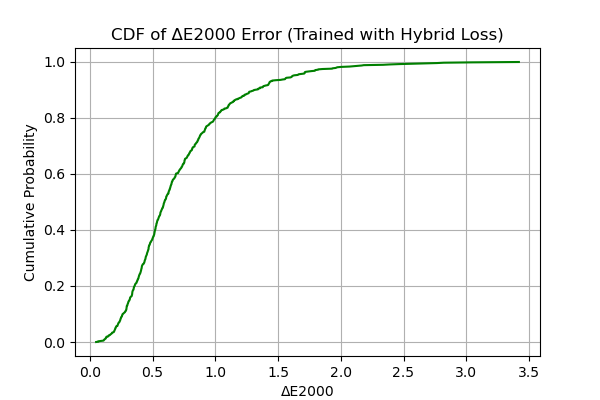
\includegraphics[width=0.8\columnwidth]{figures/CDF.png}
\bicaption[ΔE2000误差累积分布函数(混合损失训练)]{ΔE2000误差累积分布函数(混合损失训练)。}[CDF of ΔE2000 Error (Trained with Hybrid Loss)]{CDF of ΔE2000 Error (Trained with Hybrid Loss).}
\label{figure2: delta_e_cdf}
\end{figure}

从误差分析结果可以看出,直方图显示了$\Delta E_{00}$误差的分布情况,大部分预测颜色的$\Delta E_{00}$值集中在较低的范围内(例如0-2之间),这意味着模型能够很好地重现大部分目标颜色。CDF图更清晰地展示了误差的累积分布,通常认为$\Delta E_{00} < 1.0$表示人眼难以察觉的颜色差异,$\Delta E_{00} < 2.0-3.0$表示可接受的颜色差异。

\noindent\textbf{(3)色域可视化分析}

为了理解4通道输入系统和5通道输出系统各自的色域以及它们之间的关系,我们在CIE 1931色度图上绘制了它们的基色坐标点和由这些基色围成的色域(多边形)。

\begin{figure}[H]
\centering
\captionsetup{font={small, stretch=1.312}}
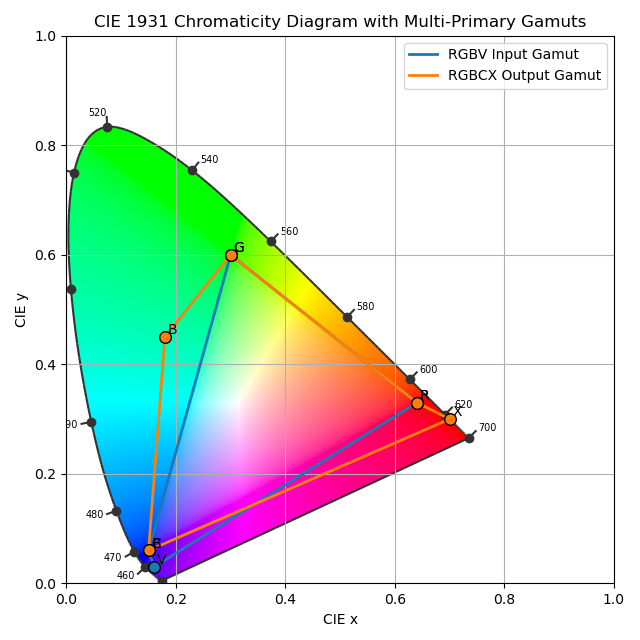
\includegraphics[width=0.67\columnwidth]{figures/色度图.png}
\bicaption[CIE 1931色度图与多基色色域]{CIE 1931色度图与多基色色域。}[CIE 1931 Chromaticity Diagram with Multi-Primary Gamuts]{CIE 1931 Chromaticity Diagram with Multi-Primary Gamuts.}
\label{figure2: chromaticity_diagram}
\end{figure}

从色域分析结果可以看出,输入色域(RGBV Input Gamut)由sRGB的R、G、B三原色以及新增的'V'(紫色)通道构成,由于'V'通道的加入,相机色域在蓝色-紫色区域得到一定的扩展。输出色域(RGBCX Output Gamut)由sRGB的R、G、B三原色,以及新增的'C'(青色)和'X'(假设更深的红色)通道构成,通过'C'和'X'的加入,显示屏的色域在蓝绿色和红色区域相对于传统sRGB显示屏得到了显著扩展。五通道显示屏的色域明显大于四通道相机的色域,这为颜色转换提供了更大的灵活性和再现能力。

\noindent\textbf{(4)样本预测效果}

为了直观地展示模型对具体颜色样本的转换效果,我们随机选择了几个验证集样本,并将其原始输入、目标输出和模型预测输出进行并排可视化。

\begin{figure}[H]
\centering
\captionsetup{font={small, stretch=1.312}}
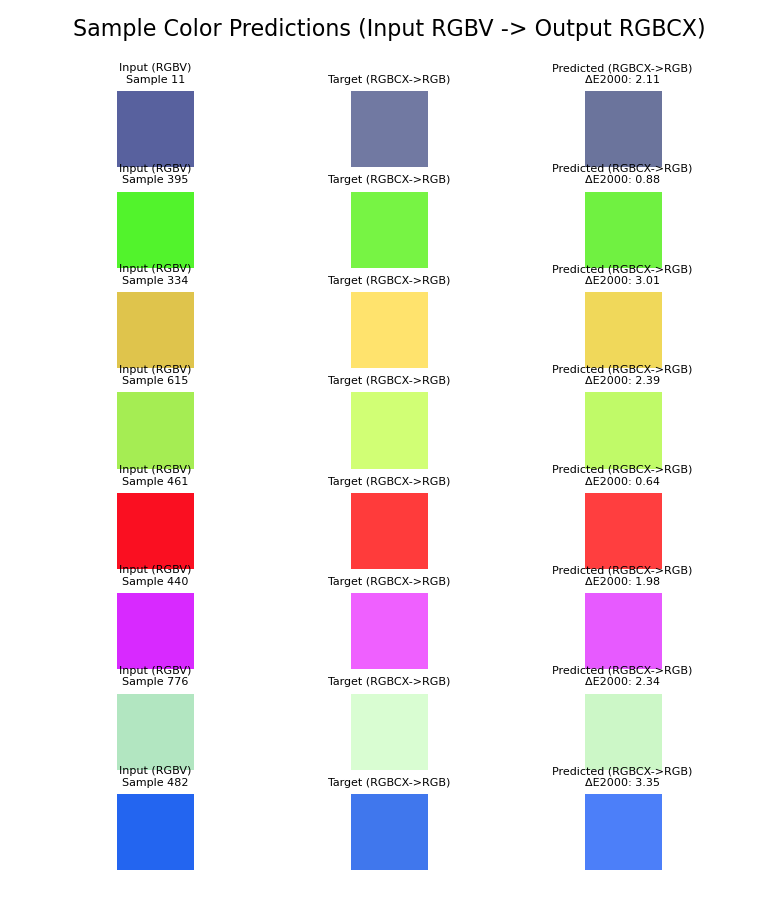
\includegraphics[width=0.8\columnwidth]{figures/Sample.png}
\bicaption[样本颜色预测(输入RGBV→输出RGBCX)]{样本颜色预测(输入RGBV→输出RGBCX)。}[Sample Color Predictions (Input RGBV → Output RGBCX)]{Sample Color Predictions (Input RGBV → Output RGBCX).}
\label{figure2: sample_predictions}
\end{figure}

每行代表一个样本:Input(RGBV)列显示了原始相机输入通过简化映射到RGB的颜色,代表了相机"看到"的颜色;Target(RGBCX->RGB)列显示了目标5通道输出通过简化映射到RGB的颜色,代表了理想情况下显示屏应该呈现的颜色;Predicted(RGBCX->RGB)列显示了模型预测的5通道输出通过简化映射到RGB的颜色,并标注了与目标颜色的$\Delta E_{00}$误差。通过对比可以看到,绝大多数样本的预测颜色与目标颜色非常接近,且$\Delta E_{00}$值较低,进一步验证了模型的有效性。

\section[\hspace{-2pt}问题3:LED显示器颜色校正模型]{{\heiti\zihao{-3} \hspace{-8pt}问题3:LED显示器颜色校正模型}}\label{section4: 问题3:LED显示器颜色校正模型}

LED显示器在实际应用中存在颜色失真问题,测量值与目标值之间存在显著偏差。本节基于CIE Lab色彩空间和三基色原理,建立了一个结合伽马校正与线性矩阵变换的颜色校正模型,通过差分进化算法优化校正参数,实现精确的颜色还原。

\subsection[\hspace{-2pt}模型建立流程]{{\heiti\zihao{4}\hspace{-8pt}模型建立流程}}\label{subsec:3-model-build}

\noindent \textbf{(1)变量定义}

\circled{1} \textbf{线性 RGB 向量}
\begin{equation}
  \mathbf{x}=\begin{bmatrix}R_\ell\\G_\ell\\B_\ell\end{bmatrix}\in[0,1]^3.
\end{equation}
其中$R_\ell, G_\ell, B_\ell$分别表示经过反伽马校正后的线性RGB分量。

\circled{2} \textbf{校正参数}
\begin{align}
  M &\in\mathbb{R}^{3\times3}, \quad \text{(校正变换矩阵)}\\
  \mathbf{b} &\in\mathbb{R}^3. \quad \text{(偏置向量)}
\end{align}

\circled{3} \textbf{校正映射}
\begin{equation}
  \mathbf{y}=\mathrm{clip}\!\bigl(M\mathbf{x}+\mathbf{b},[0,1]\bigr).
\end{equation}
该映射确保输出值域限制在有效的RGB范围内。

\noindent\textbf{(2)伽马校正模型}

基于第\ref{chapter3: 理论基础}章中建立的伽马校正理论(见第\ref{section2: 伽马校正理论}节),对每个颜色通道$c \in \{R,G,B\}$,建立响应关系:
\begin{equation}
  I_{\text{meas},c} = S_c \cdot (I_{\text{target},c})^{\gamma_c}
\end{equation}
其中$\gamma_c$为伽马值,$S_c$为比例因子。

通过对三种基色图像的实际测量数据进行伽马参数估计,采用对数线性回归方法(详见第\ref{subsection2: 伽马参数估计}节),得到的结果如表\ref{table:gamma_params}所示:

\begin{table}[h!]
\small    % 设置表格字体为5号
\setstretch{1.245}        % 设置具有指定弹力的橡皮长度(原行宽的1.2倍)
\captionsetup{font={small, stretch=1.512}}
\centering
\bicaption[不同基色图像的伽马参数估计结果]{不同基色图像的伽马参数估计结果。}[Gamma parameter estimation results for different primary color images]{Gamma parameter estimation results for different primary color images.}    % 中英文标题
\begin{tabularx}{\textwidth}{lCCCCCC}
\toprule
\multirow{2}{*}{图像类型} & \multicolumn{3}{c}{伽马值 ($\gamma_c$)} & \multicolumn{3}{c}{比例因子 ($S_c$)} \\
\cline{2-7}
 & \raisebox{-2pt}{R通道} & \raisebox{-2pt}{G通道} & \raisebox{-2pt}{B通道} & \raisebox{-2pt}{R通道} & \raisebox{-2pt}{G通道} & \raisebox{-2pt}{B通道} \\
\midrule
红色图像 & 0.022 & 0.229 & 0.230 & 0.862 & 0.988 & 0.988 \\
绿色图像 & 0.228 & 0.022 & 0.232 & 0.988 & 0.862 & 0.987 \\
蓝色图像 & 0.231 & 0.228 & 0.022 & 0.988 & 0.988 & 0.861 \\
\bottomrule
\end{tabularx}
%\vspace{-20pt}
\label{table:gamma_params}
\end{table}

从伽马参数估计结果可以观察到一个重要现象:主色通道(红色图像的R通道、绿色图像的G通道、蓝色图像的B通道)的伽马值显著较小(约0.022),而非主色通道的伽马值相对较大(约0.23)。这表明LED显示器在显示主色时存在更强的非线性响应特性,需要更大的校正幅度。

根据第\ref{subsection2: 伽马校正变换}节中的伽马校正变换公式,线性化变换为:
\begin{align}
  \text{前向:} \quad &I_{\text{out}} = \text{clip}((I_{\text{in}} \cdot S)^{\gamma}, [0,1])\\
  \text{反向:} \quad &I_{\text{out}} = \text{clip}((I_{\text{in}})^{1/\gamma} / S, [0,1])
\end{align}

\noindent\textbf{(3)目标函数设计}

我们设计了一个综合的目标函数,包含多个组成部分以确保校正效果的全面性。

首先是色差损失,基于第\ref{section2: CIEDE2000色差公式}节中的CIE $\Delta E_{00}$色差公式构建目标函数:
\begin{equation}
L_{\mathrm{DE}}=\frac{1}{N}\sum_{k=1}^N \Delta E_{00}\!\bigl(\mathbf{L}_{\mathrm{t},k},\mathbf{L}_{\mathrm{c},k}\bigr)
\end{equation}
其中$\mathbf{L}_{\mathrm{t},k}$和$\mathbf{L}_{\mathrm{c},k}$分别表示第$k$个像素点的目标和校正后的CIE Lab值(Lab空间转换详见第\ref{section2: CIELab颜色空间}节)。

其次是正则化项:
\begin{equation}
L_{\mathrm{reg}}=\lambda_1\|M-I_3\|_F^2+\lambda_2\|\mathbf{b}\|_2^2
\end{equation}
用于防止校正矩阵过度偏离单位矩阵,确保变换的稳定性。

同时引入行列式惩罚:
\begin{equation}
L_{\det}=\lambda_3 \cdot \mathbf{1}\bigl(\det M\leq0 \lor |\det M|<\epsilon\bigr)
\end{equation}
其中$\epsilon=0.1$,确保变换矩阵的可逆性和数值稳定性。

最终的总目标函数为:
\begin{equation}
\mathcal{L}(M,\mathbf{b})=L_{\mathrm{DE}}+L_{\mathrm{reg}}+L_{\det}
\end{equation}
参数设置为$\lambda_1=\lambda_2=0.001$,$\lambda_3=1000$。

该目标函数综合考虑了颜色感知准确性、数值稳定性和矩阵可逆性,其中RGB到XYZ到Lab的完整转换流程详见第\ref{subsection2: CIE1931标准色度观察者与XYZ颜色空间}节和第\ref{subsection2: CIELab颜色空间}节。

\subsection[\hspace{-2pt}模型求解策略]{{\heiti\zihao{4}\hspace{-8pt}模型求解策略}}\label{subsec:3-solver}

考虑到目标函数的非凸性和多模态特征,采用全局-局部混合优化策略:

\noindent\textbf{(1)差分进化全局搜索}

\circled{1} \textbf{参数空间设定}

在参数空间$\{M_{ij}\in[-2,2],\,b_i\in[-0.1,0.1]\}$内进行全局搜索:
\begin{align}
  \text{种群大小:} &\quad \text{popsize} = 15\\
  \text{最大迭代:} &\quad \text{maxiter} = 200\\
  \text{变异因子:} &\quad F \in [0.5, 2.0]\\
  \text{交叉概率:} &\quad CR = 0.7
\end{align}
得到初值$\theta_0=(\operatorname{vec}(M_0),\mathbf{b}_0)$。

\circled{2} \textbf{差分进化操作}

通过经典的种群初始化、变异、交叉及选择等核心操作,DE算法能够迭代地搜寻旨在最小化以 $\Delta E_{00}$ 度量的感知色彩差异的解。

\noindent\textbf{(2)L-BFGS-B局部精调}

\circled{1} \textbf{局部优化设置}

以$\theta_0$为起点,采用拟牛顿法进行局部优化:
\begin{equation}
  (M^*,\mathbf{b}^*) = \arg\min_{M,\mathbf{b}} \mathcal{L}(M,\mathbf{b})
\end{equation}
\begin{align}
  \text{最大迭代:} &\quad 500\\
  \text{收敛容差:} &\quad 10^{-6}\\
  \text{梯度容差:} &\quad 10^{-5}
\end{align}

\noindent\textbf{(3)算法流程}

\circled{1} \textbf{完整算法描述}

\begin{algorithm}[H]\small
\setstretch{1.245} %设置具有指定弹力的橡皮长度(原行宽的1.2倍)
\renewcommand{\algorithmcfname}{算法}
	\caption{LED颜色校正算法}
	\KwIn{测量数据$\mathbf{X}_{\text{meas}} \in \mathbb{R}^{H \times W \times 3}$,目标数据$\mathbf{X}_{\text{target}} \in \mathbb{R}^{H \times W \times 3}$}
	\KwOut{校正矩阵$M^*$,偏置向量$\mathbf{b}^*$}
	
	\textbf{步骤1:伽马参数估计}\\
	\For{$c \in \{R,G,B\}$}{
		提取通道数据:$I_{\text{meas},c}$, $I_{\text{target},c}$\\
		拟合:$\log(I_{\text{meas},c}) = \gamma_c \log(I_{\text{target},c}) + \log(S_c)$\\
		求解:$\gamma_c$, $S_c$\\
	}
	
	\textbf{步骤2:数据预处理}\\
	反伽马校正:$\mathbf{X}_{\text{meas,lin}} \leftarrow \Gamma^{-1}(\mathbf{X}_{\text{meas}})$\\
	反伽马校正:$\mathbf{X}_{\text{target,lin}} \leftarrow \Gamma^{-1}(\mathbf{X}_{\text{target}})$\\
	
	\textbf{步骤3:全局优化}\\
	初始化DE种群:$\mathcal{P}_0 = \{\theta_1, \theta_2, \ldots, \theta_{\text{popsize}}\}$\\
	\For{$t = 1$ \textbf{to} $\text{maxiter}$}{
		\For{每个个体$\theta_i \in \mathcal{P}_t$}{
			变异:$\mathbf{v}_i = \theta_{r1} + F \cdot (\theta_{r2} - \theta_{r3})$\\
			交叉:$\mathbf{u}_i = \text{crossover}(\theta_i, \mathbf{v}_i, CR)$\\
			选择:$\theta_i^{t+1} = \arg\min_{\{\theta_i, \mathbf{u}_i\}} \mathcal{L}(\cdot)$\\
		}
	}
	获得最优个体:$\theta_0 = \arg\min_{\theta \in \mathcal{P}_{\text{final}}} \mathcal{L}(\theta)$\\
	
	\textbf{步骤4:局部精调}\\
	$(M^*, \mathbf{b}^*) \leftarrow \text{L-BFGS-B}(\theta_0, \mathcal{L})$\\
	
	\label{algorithm:led_correction}
\end{algorithm}
\vspace{20pt}

\noindent\textbf{(4)校正应用流程}

完整的颜色校正应用流程包括三个主要步骤:首先对输入sRGB进行反伽马校正,即线性化处理$\mathbf{x}_\ell = \Gamma^{-1}(\mathbf{x}_{\mathrm{srgb}})$;然后应用校正矩阵和偏置进行线性变换$\mathbf{y}_\ell = \mathrm{clip}\!\bigl(M^*\mathbf{x}_\ell+\mathbf{b}^*,[0,1]\bigr)$;最后进行正向伽马校正,重新编码恢复到sRGB空间$\mathbf{y}_{\mathrm{srgb}}=\Gamma(\mathbf{y}_\ell)$。

\subsection[\hspace{-2pt}模型验证与分析]{{\heiti\zihao{4}\hspace{-8pt}模型验证与分析}}\label{subsec:3-validation}

\noindent\textbf{(1)可视化结果分析}

\circled{1} \textbf{RGB通道校正对比}

\begin{figure}[H]
  \centering
  \captionsetup{font={small, stretch=1.312}}

  \begin{subfigure}[b]{0.6\textwidth}
    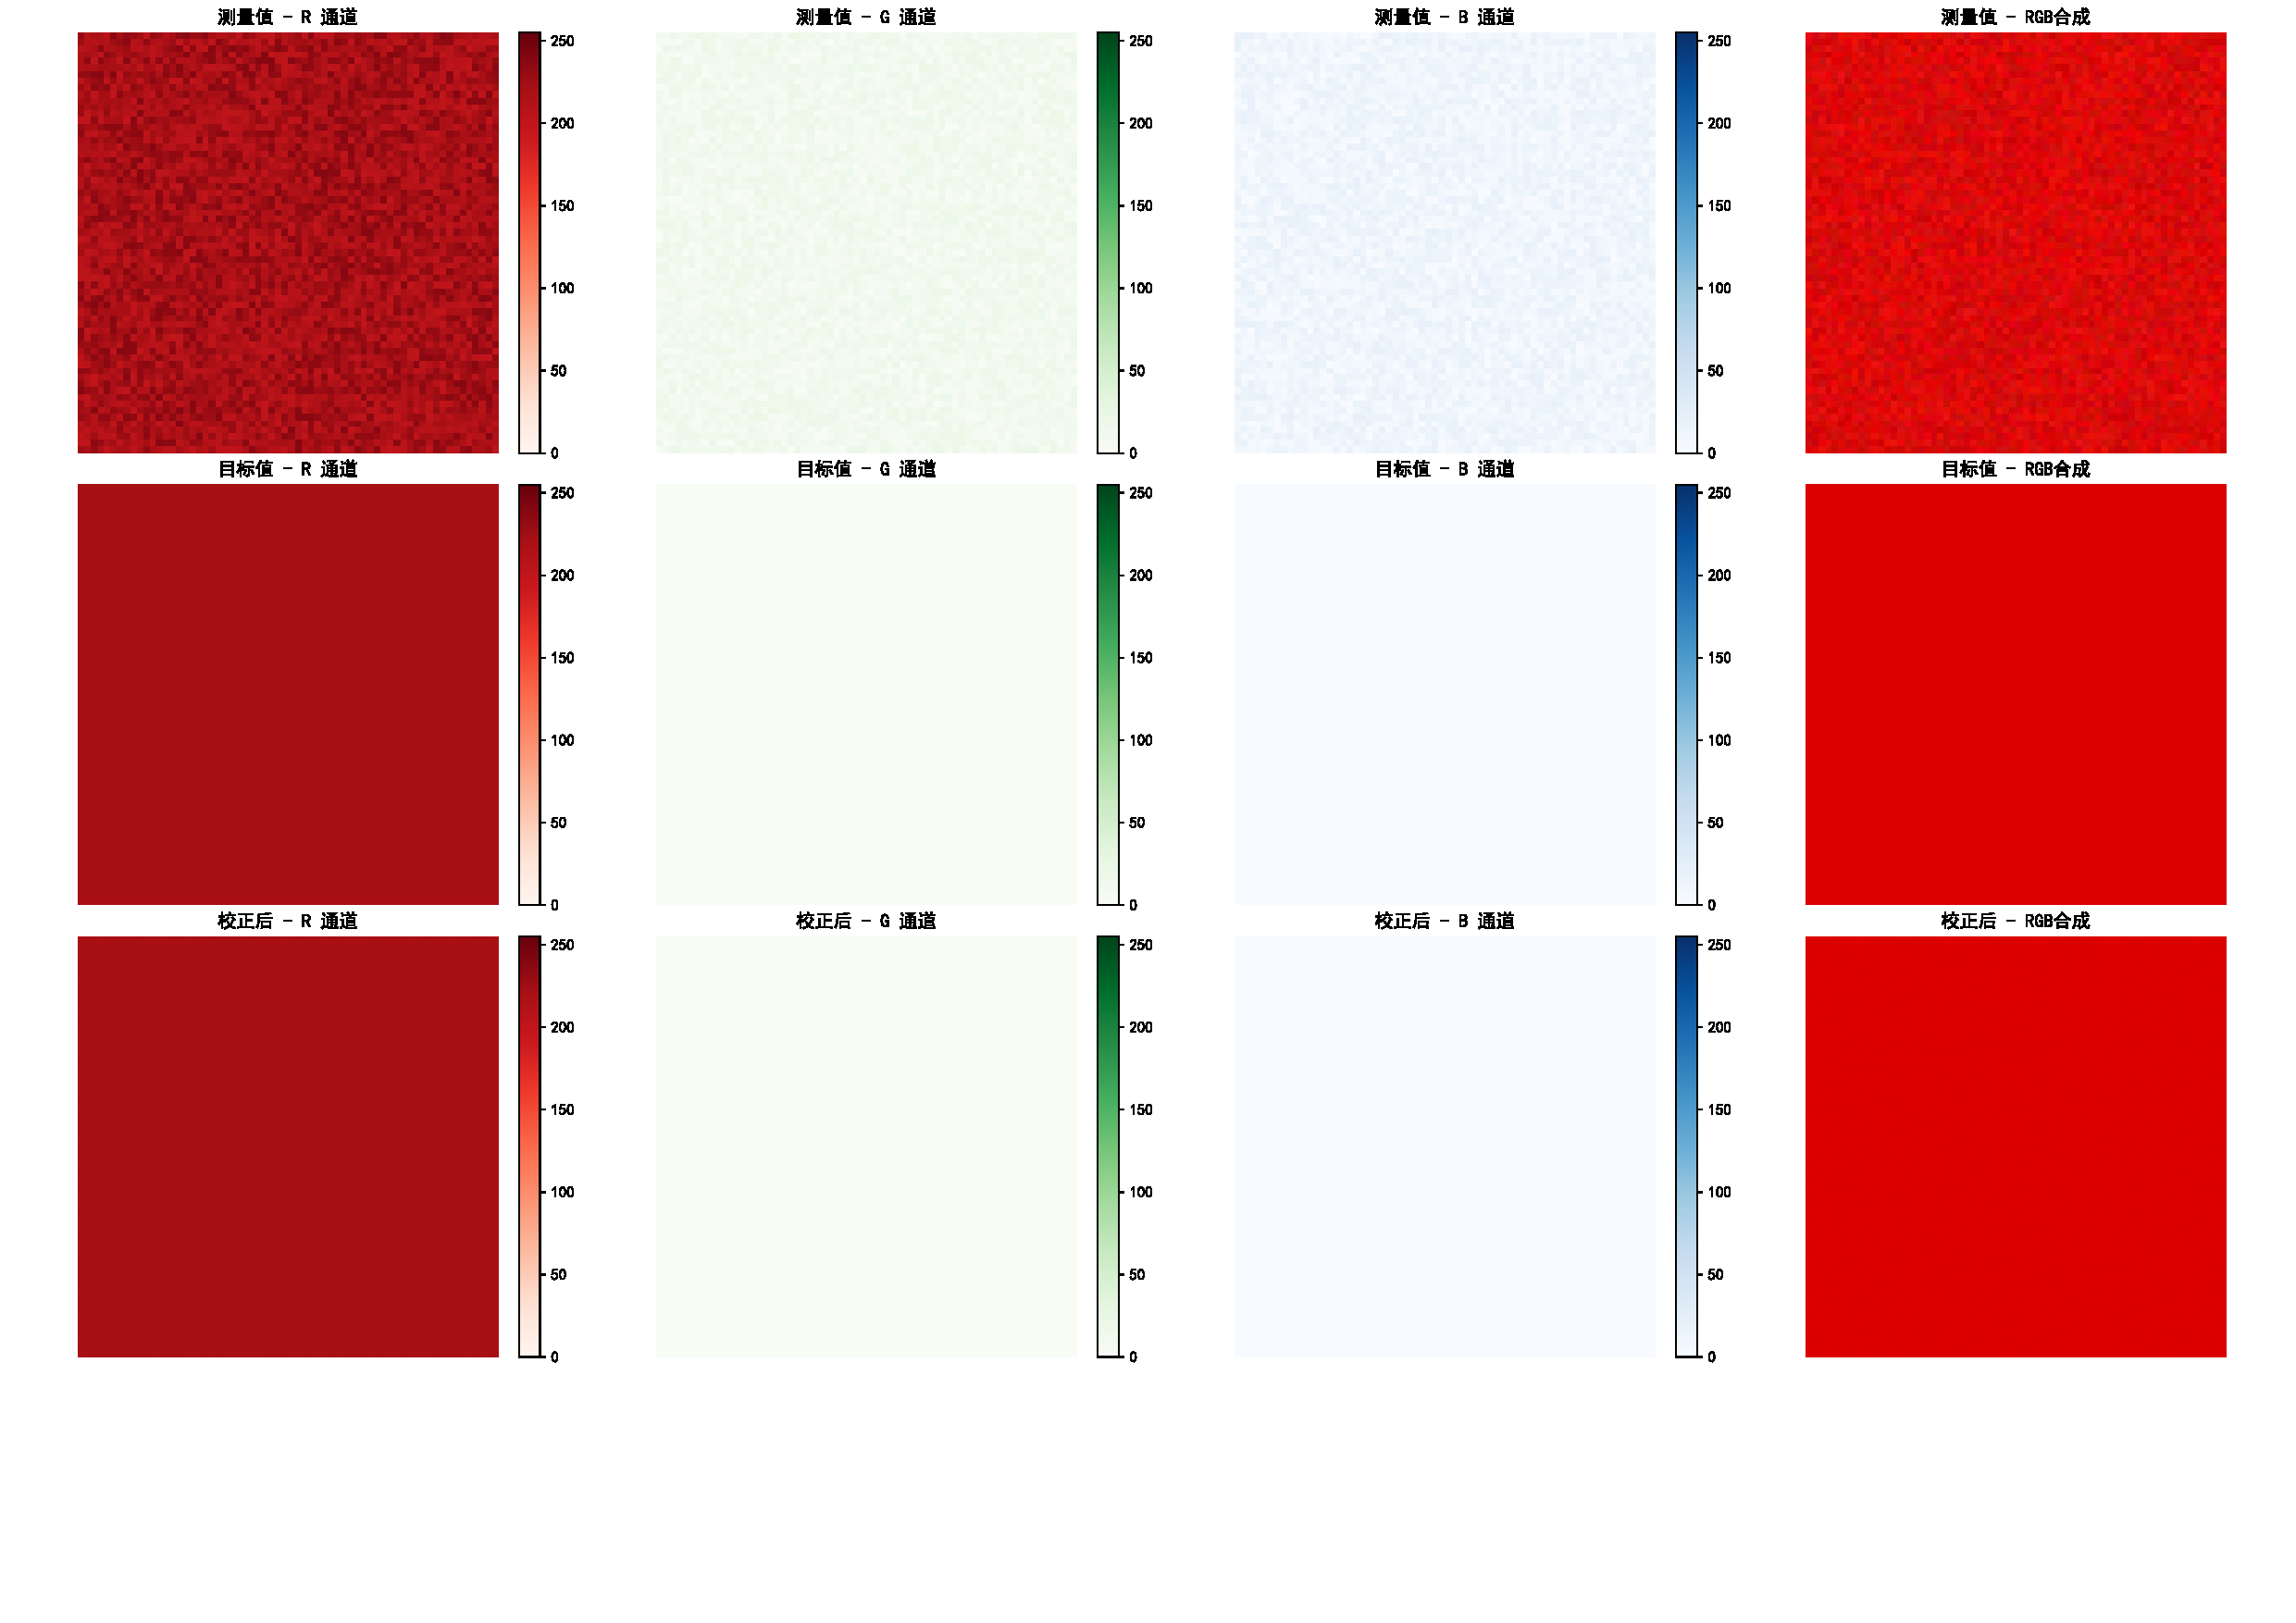
\includegraphics[width=\textwidth]{figures/model_solution/p3/R.pdf}
    \bicaption[红色图片各通道校正前后对比示意图]
        {红色图片各通道校正前后对比示意图。}[Comparison of pre- and post-correction for red image channels]{Comparison of pre- and post-correction for red image channels.}
    \label{figure4:r_compare}
  \end{subfigure}
  \hfill
  \begin{subfigure}[b]{0.6\textwidth}
    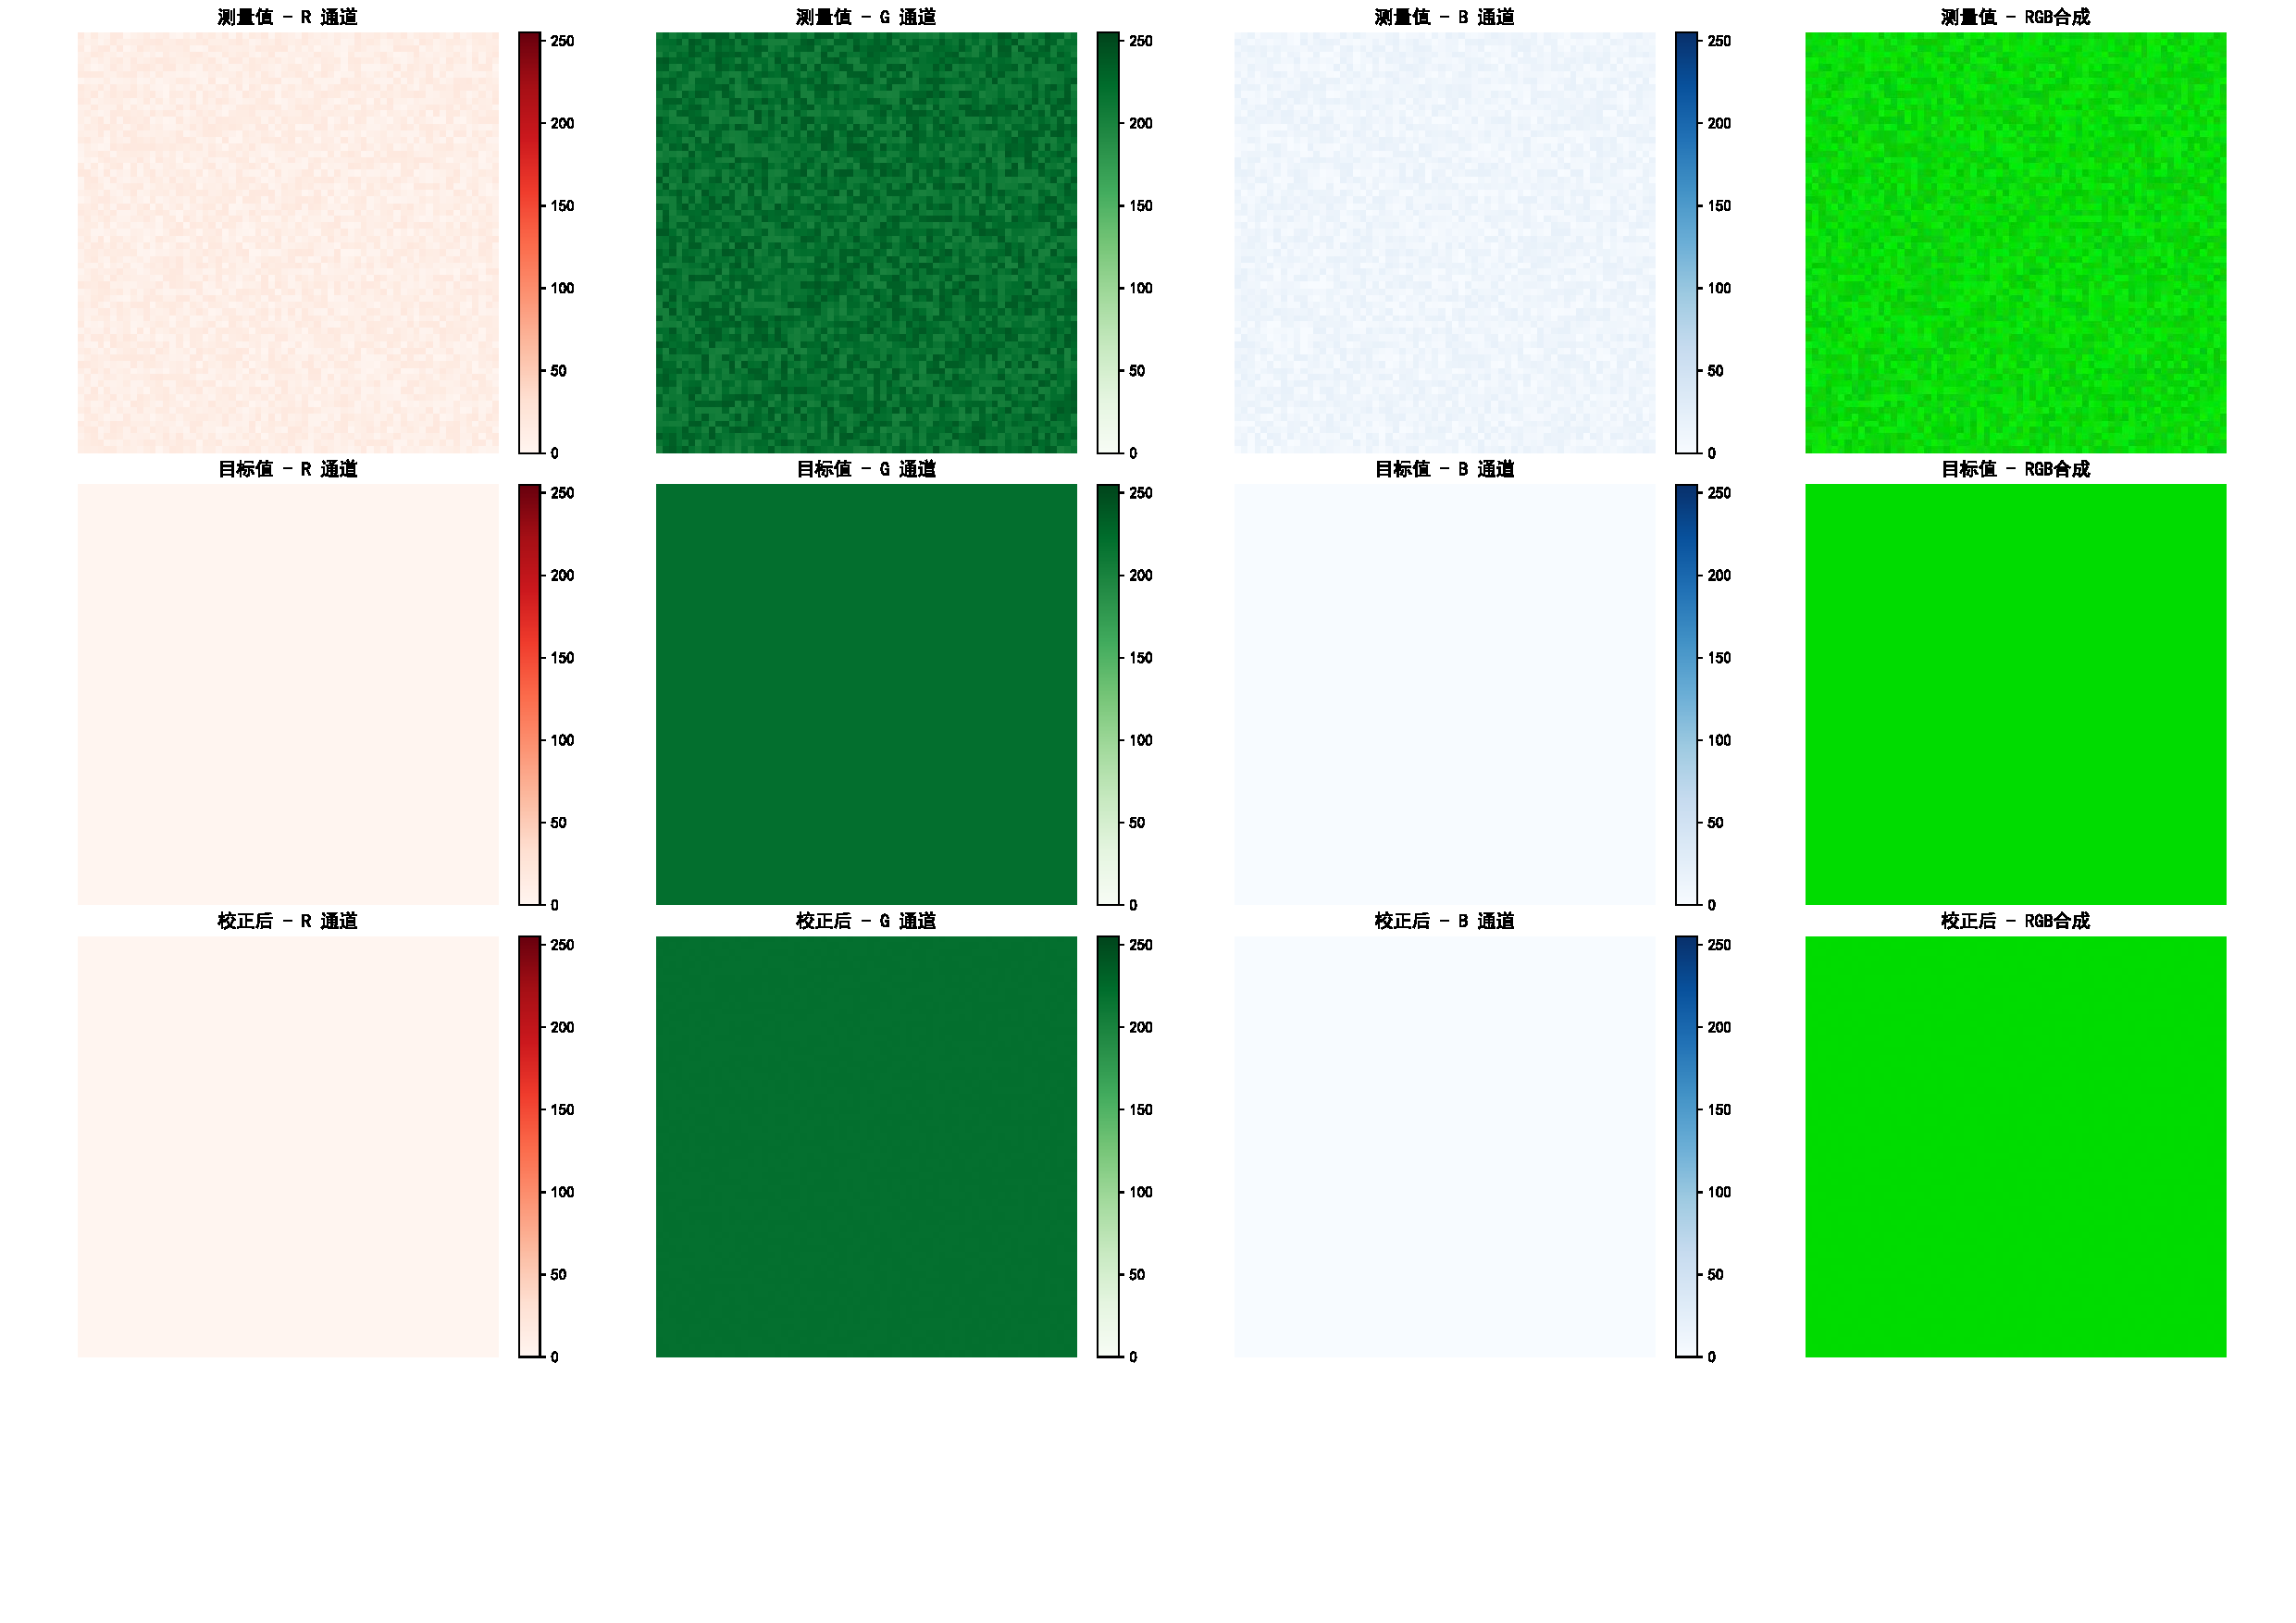
\includegraphics[width=\textwidth]{figures/model_solution/p3/G.pdf}
    \bicaption[绿色图片各通道校正前后对比示意图]
        {绿色图片各通道校正前后对比示意图。}[Comparison of pre- and post-correction for green image channels]{Comparison of pre- and post-correction for green image channels.}
    \label{figure4:g_compare}
  \end{subfigure}
  \hfill
  \begin{subfigure}[b]{0.6\textwidth}
    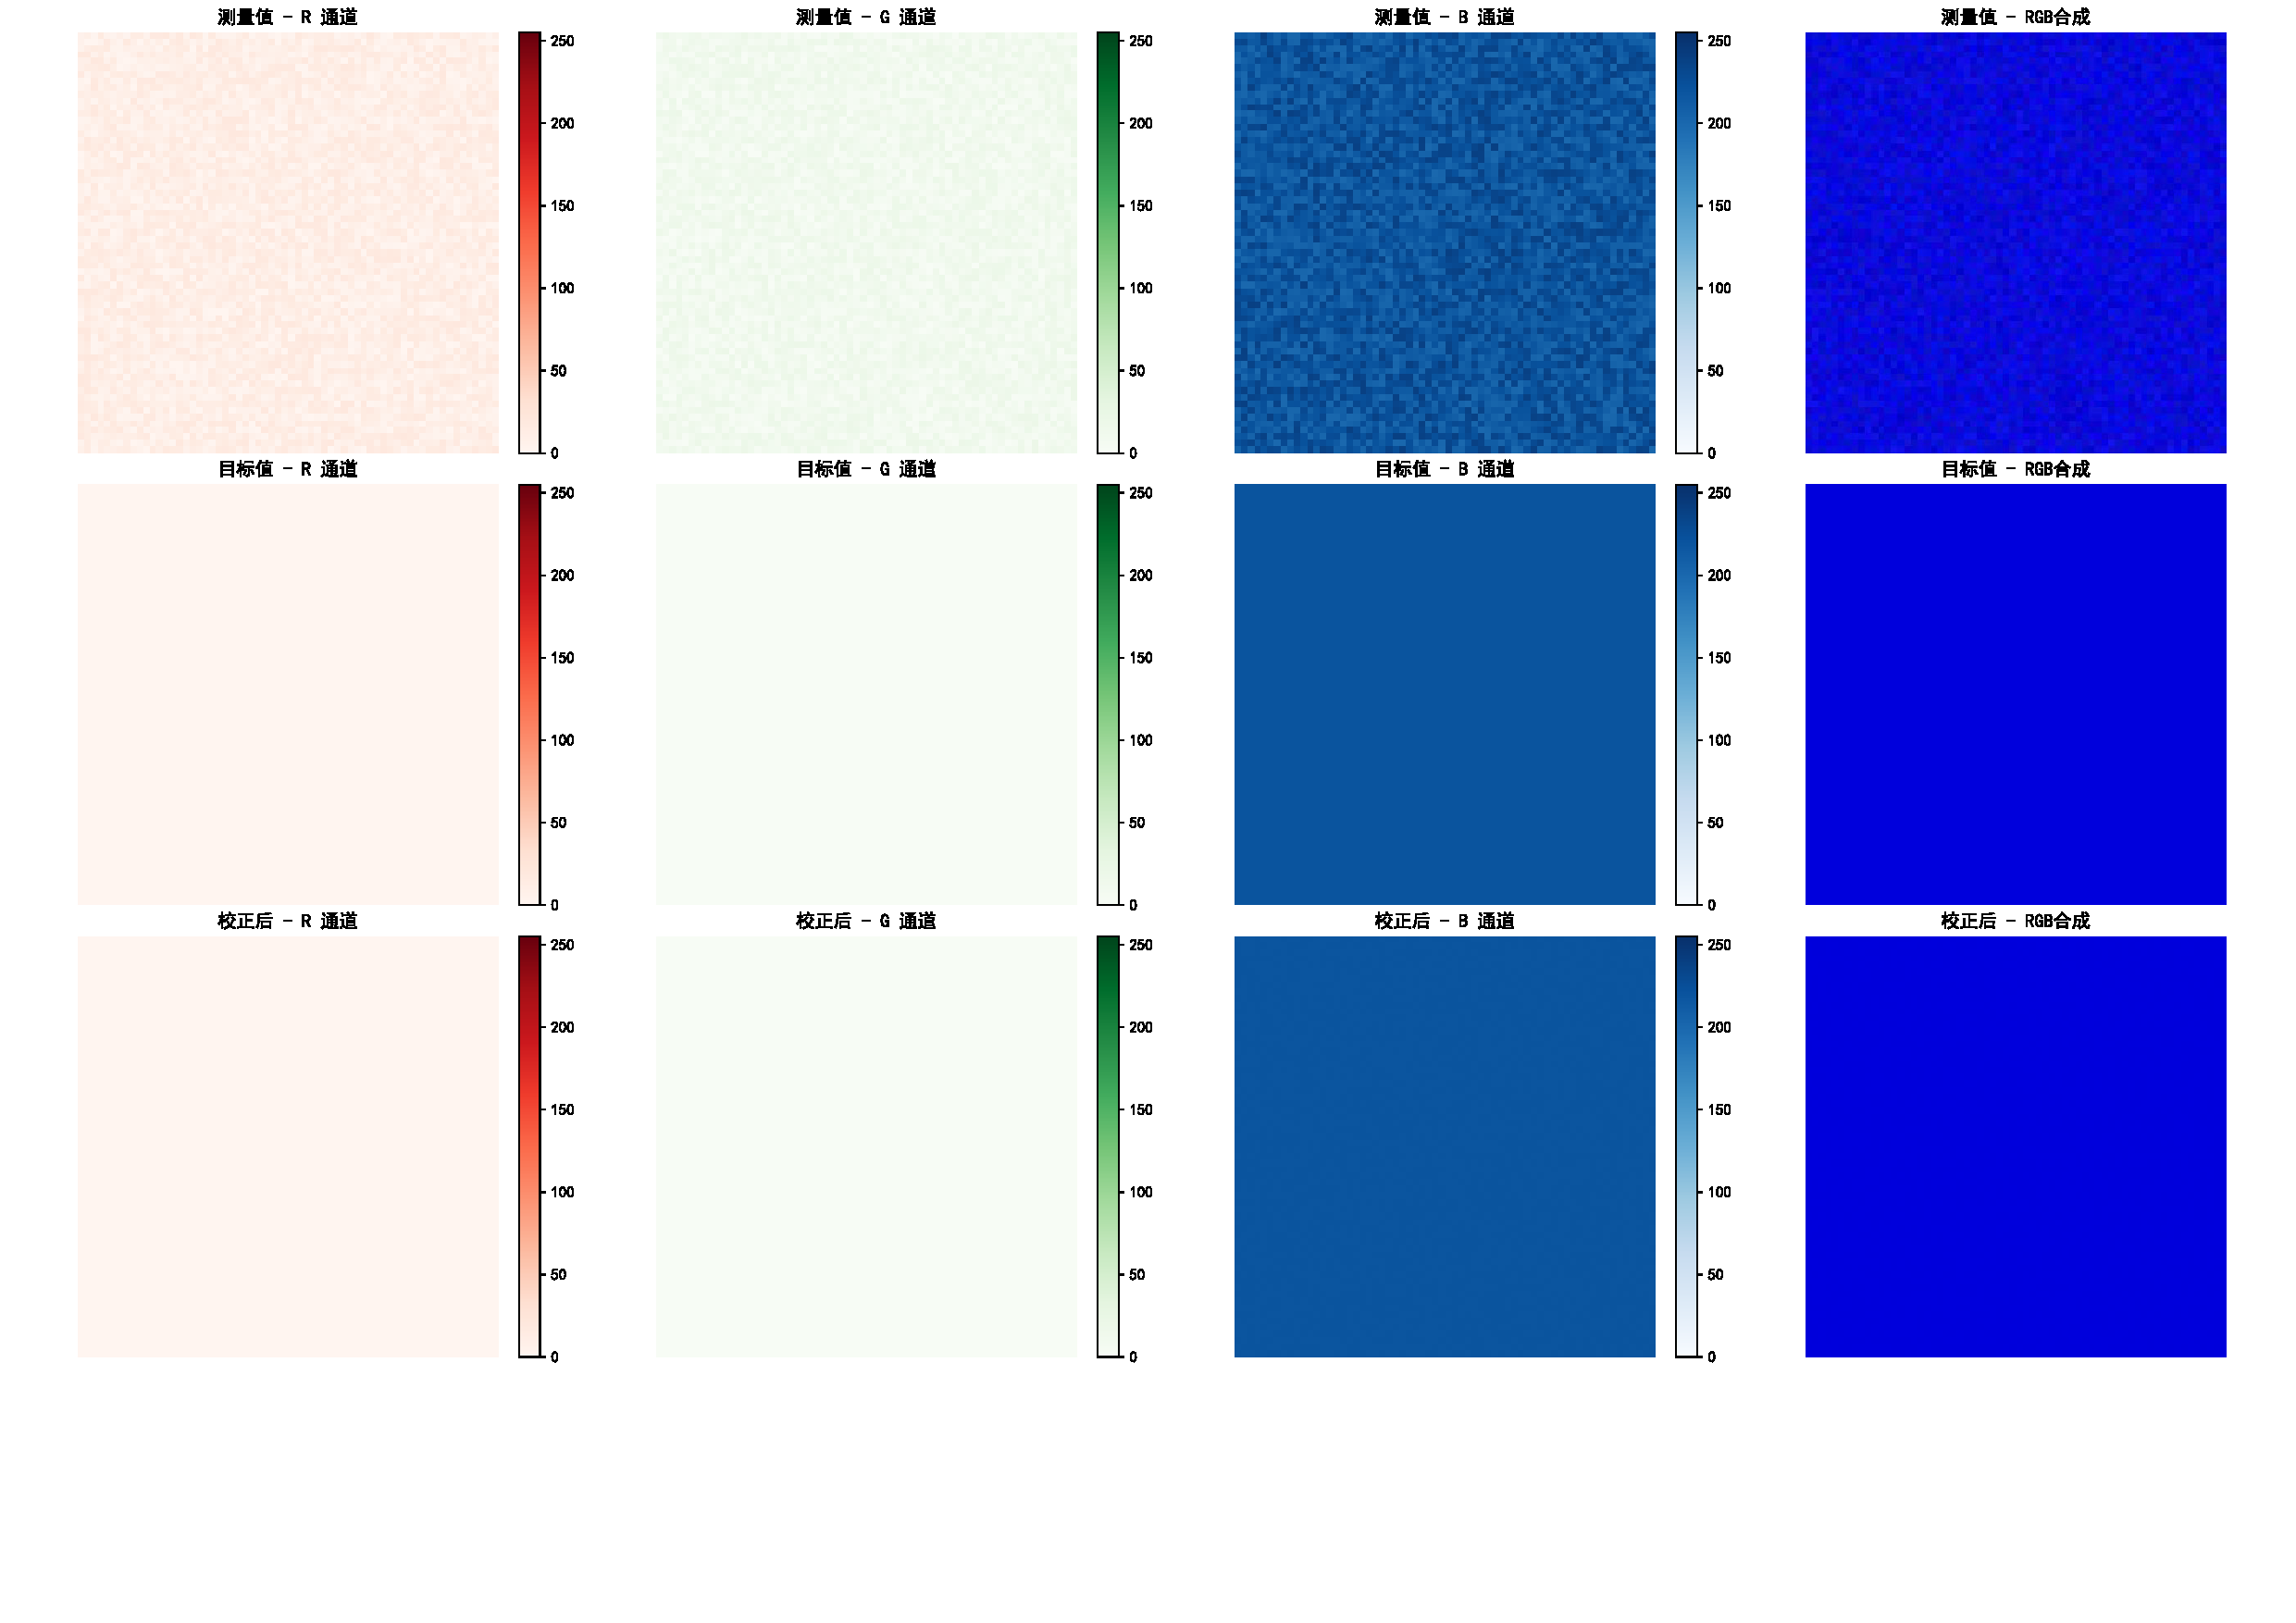
\includegraphics[width=\textwidth]{figures/model_solution/p3/B.pdf}
    \bicaption[蓝色图片各通道校正前后对比示意图]
        {蓝色图片各通道校正前后对比示意图。}[Comparison of pre- and post-correction for blue image channels]{Comparison of pre- and post-correction for blue image channels.}
    \label{figure4:b_compare}
  \end{subfigure}

  \bicaption[RGB三原色图像校正前后对比示意图]{RGB三原色图像校正前后对比示意图。}[Comparison of Pre- and Post-Correction for RGB Channels]{Comparison of Pre- and Post-Correction for RGB Channels.}
  \label{figure4:rgb_compare}
\end{figure}

通过可视化分析可以观察到,校正后的图像在色彩还原度和视觉效果方面均有显著改善,RGB各通道的分布更接近目标值。

\noindent\textbf{(2)定量评估结果}

基于CIE $\Delta E_{00}$色差评估标准,我们对三种基色图像(红色、绿色、蓝色)分别进行了颜色校正实验。表\ref{table:correction_results}展示了详细的定量评估结果。

\begin{table}[h!]
\small    % 设置表格字体为5号
\setstretch{1.245}        % 设置具有指定弹力的橡皮长度(原行宽的1.2倍)
\captionsetup{font={small, stretch=1.512}}
\centering
\bicaption[LED颜色校正效果定量评估结果]{LED颜色校正效果定量评估结果。}[Quantitative evaluation results of LED color correction]{Quantitative evaluation results of LED color correction.}    % 中英文标题
\begin{tabularx}{\textwidth}{lCCCC}
\toprule
评估指标 & 红色图像 & 绿色图像 & 蓝色图像 & 平均值 \\
\midrule
校正前平均色差 $\overline{\Delta E}_{00}^{\text{before}}$ & 2.540 & 2.418 & 1.519 & 2.159 \\
校正后平均色差 $\overline{\Delta E}_{00}^{\text{after}}$ & 0.106 & 0.115 & 0.063 & 0.095 \\
色差改善值 & 2.434 & 2.303 & 1.456 & 2.064 \\
改善百分比 & 95.8\% & 95.2\% & 95.9\% & 95.6\% \\
校正前最大色差 & 5.207 & 5.015 & 3.344 & 4.522 \\
校正后最大色差 & 0.212 & 0.236 & 0.128 & 0.192 \\
色差<1.0像素比例(校正前) & 9.0\% & 20.9\% & 24.9\% & 18.3\% \\
色差<1.0像素比例(校正后) & 100.0\% & 100.0\% & 100.0\% & 100.0\% \\
校正矩阵行列式值 & 0.100 & 0.103 & 0.100 & 0.101 \\
\bottomrule
\end{tabularx}
%\vspace{-20pt}
\label{table:correction_results}
\end{table}

从定量评估结果可以看出,该模型在颜色校正精度方面表现优异:

\textbf{色差改善效果显著}:三种基色图像的平均色差均从2.0以上降低到0.1左右,平均改善幅度达到95.6\%,表明校正效果非常显著。校正后的平均色差均小于0.12,远低于人眼可察觉的色差阈值(通常认为$\Delta E_{00} < 1.0$表示难以察觉的差异)。

\textbf{极值控制良好}:校正前的最大色差在3.3-5.2之间,校正后均控制在0.25以下,最大色差的改善幅度超过95\%,说明模型不仅改善了整体色差,也有效控制了极端偏差。

\textbf{像素级精度提升}:校正前色差小于1.0的像素比例仅为9.0\%-24.9\%,校正后所有像素的色差均小于1.0,达到100\%的优秀覆盖率,表明校正效果在像素级别上的一致性。

\textbf{数值稳定性验证}:所有校正矩阵的行列式值均在0.10左右,远大于设定的阈值$\epsilon=0.1$,验证了变换矩阵的数值稳定性和可逆性,确保了校正过程的数学可靠性。

\textbf{伽马参数分析}:从实验结果可以观察到,主色通道(如红色图像的R通道、绿色图像的G通道、蓝色图像的B通道)的伽马值显著较小(约0.022),而其他通道的伽马值相对较大(约0.23),这反映了LED显示器在不同颜色通道上的非线性响应特性差异。

\textbf{校正参数分析}:表\ref{table:bias_vectors}展示了三种基色图像优化得到的偏置向量,这些参数反映了LED显示器在不同颜色显示时的系统性偏差。

\begin{table}[h!]
\small    % 设置表格字体为5号
\setstretch{1.245}        % 设置具有指定弹力的橡皮长度(原行宽的1.2倍)
\captionsetup{font={small, stretch=1.512}}
\centering
\bicaption[不同基色图像的校正偏置向量]{不同基色图像的校正偏置向量。}[Correction bias vectors for different primary color images]{Correction bias vectors for different primary color images.}    % 中英文标题
\begin{tabularx}{\textwidth}{lCCC}
\toprule
图像类型 & R通道偏置 & G通道偏置 & B通道偏置 \\
\midrule
红色图像 & 0.00135 & -0.01465 & -0.02861 \\
绿色图像 & -0.06570 & 0.00137 & -0.08602 \\
蓝色图像 & -0.05301 & -0.04425 & 0.00149 \\
\bottomrule
\end{tabularx}
%\vspace{-20pt}
\label{table:bias_vectors}
\end{table}

从偏置向量分析可以看出,主色通道的偏置值相对较小(接近0),而非主色通道需要较大的负偏置校正,这表明LED显示器在显示非主色时存在系统性的过度响应,需要通过负偏置进行抑制。

\noindent\textbf{(3)模型特点总结}

本模型具有以下显著特点:在理论完备性方面,基于CIE Lab色彩空间的感知均匀性,采用$\Delta E_{00}$色差公式,符合人眼视觉特性;在数值稳定性方面,通过正则化项和行列式约束,确保校正矩阵的条件数适中,避免数值不稳定;在优化鲁棒性方面,差分进化与梯度方法的混合策略,平衡了全局搜索能力和局部收敛效率;在实用性方面,校正流程简洁高效,适合实时颜色校正应用。